\documentclass[12pt]{report}
\usepackage[utf8]{inputenc}
\usepackage[russian]{babel}
%\usepackage[14pt]{extsizes}
\usepackage{listings}
\usepackage{graphicx}
\usepackage{amsmath,amsfonts,amssymb,amsthm,mathtools} 
\usepackage{pgfplots}
\usepackage{filecontents}
\usepackage{indentfirst}
\usepackage{eucal}
\usepackage{float} 
\usepackage{amsmath}
\usepackage{enumitem}
\usepackage[justification=centering]{caption} 
\usepackage{tikz}
\usepackage{pgfplots}
\pgfplotsset{compat=newest}

\frenchspacing

\usepackage{indentfirst} % Красная строка


%\usetikzlibrary{datavisualization}
%\usetikzlibrary{datavisualization.formats.functions}

\usepackage{amsmath}


% Для листинга кода:
\lstset{ %
	language=haskell,                 % выбор языка для подсветки (здесь это С)
	basicstyle=\small\sffamily, % размер и начертание шрифта для подсветки кода
	numbers=left,               % где поставить нумерацию строк (слева\справа)
	numberstyle=\tiny,           % размер шрифта для номеров строк
	stepnumber=1,                   % размер шага между двумя номерами строк
	numbersep=5pt,                % как далеко отстоят номера строк от подсвечиваемого кода
	showspaces=false,            % показывать или нет пробелы специальными отступами
	showstringspaces=false,      % показывать или нет пробелы в строках
	showtabs=false,             % показывать или нет табуляцию в строках
	frame=single,              % рисовать рамку вокруг кода
	tabsize=2,                 % размер табуляции по умолчанию равен 2 пробелам
	captionpos=t,              % позиция заголовка вверху [t] или внизу [b] 
	breaklines=true,           % автоматически переносить строки (да\нет)
	breakatwhitespace=false, % переносить строки только если есть пробел
	escapeinside={\#*}{*)}   % если нужно добавить комментарии в коде
}

\usepackage[left=2cm,right=2cm, top=2cm,bottom=2cm,bindingoffset=0cm]{geometry}

\usepackage{listings}

\usepackage{titlesec}
\titleformat{\section}
{\normalsize\bfseries}
{\thesection}
{1em}{}
\titlespacing*{\chapter}{0pt}{-30pt}{8pt}
\titlespacing*{\section}{\parindent}{*4}{*4}
\titlespacing*{\subsection}{\parindent}{*4}{*4}
\usepackage{setspace}

\titleformat{\chapter}{\LARGE\bfseries}{\thechapter}{20pt}{\large\bfseries}
\titleformat{\section}{\Large\bfseries}{\thesection}{20pt}{\large\bfseries}

\makeatletter 

\begin{document}
	
%\def\chaptername{} % убирает "Глава"
\thispagestyle{empty}
\begin{titlepage}
	\noindent \begin{minipage}{0.15\textwidth}
		
\includegraphics[width=\linewidth]{pics/logo}
	\end{minipage}
	\noindent\begin{minipage}{0.9\textwidth}\centering
		\textbf{Министерство науки и высшего образования Российской Федерации}\\
		\textbf{Федеральное государственное бюджетное образовательное учреждение высшего образования}\\
		\textbf{~~~«Московский государственный технический университет имени Н.Э.~Баумана}\\
		\textbf{(национальный исследовательский университет)»}\\
		\textbf{(МГТУ им. Н.Э.~Баумана)}
	\end{minipage}
	
	\noindent\rule{18cm}{3pt}
	\newline\newline
	\noindent ФАКУЛЬТЕТ $\underline{\text{«Информатика и системы управления»}}$ \newline\newline
	\noindent КАФЕДРА $\underline{\text{«Программное обеспечение ЭВМ и информационные технологии»}}$\newline\newline\newline\newline\newline
	
	
	\begin{center}
		\noindent\begin{minipage}{1.3\textwidth}\centering
			\Large\textbf{  Отчёт по лабораторной работе №1 по курсу}\newline\newline
			\textbf{<<Математическая статистика>>}\newline
		\end{minipage}
	\end{center}
	
	~\\\\\\\\\\
	\large
	\noindent\textbf{Тема } $\underline{\text{Гистограмма и эмпирическая функция распределения.}}$\newline\newline
	\noindent\textbf{Студент } $\underline{\text{Сироткина П.Ю.}}$\newline\newline
	\noindent\textbf{Номер варианта} $\underline{\text{~~~12~~~}}$\newline\newline
	\noindent\textbf{Группа } $\underline{\text{ИУ7-66Б}}$\newline\newline
	\noindent\textbf{Преподаватель } $\underline{\text{Андреева Т.В.}}$\newline\newline
	\noindent\textbf{Оценка } $\underline{\text{~~~~~~~~~~~~~~~~~~~~~~~~~}}$\newline\newline
	
	\begin{center}
		\vfill
		Москва~---~\the\year
		~г.
	\end{center}
\end{titlepage}

\section*{1. Цель работы}

Построение гистограммы и эмпирической функции распределения.

~\

\section*{2. Постановка задачи}

\begin{enumerate}
	\item Для выборки объема $n$ из генеральной совокупности $X$ реализовать в виде программы на ЭВМ:
		\begin{enumerate}
			\item вычисление максимального значения $M_{max}$ и минимального значения $M_{min}$;
			\item размаха R выборки;
			\item вычисление оценок $\hat\mu$ и $S^2$ математического ожидания $MX$ и дисперсии $DX$;
			\item группировку значений выборки в $m = [log_2n] + 2$ интервала;
			\item построение на одной координатной плоскости гистограммы и графика функции плотности распределения вероятностей нормальной случайной величины с математическим ожиданием $\hat\mu$ и дисперсией $S^2$;
			\item построение на другой координатной плоскости графика эмпирической функции распределения и функции распределения нормальной случайной величины с математическим ожиданием $\hat\mu$ и дисперсией $S^2$.
		\end{enumerate}
	\item Провести вычисления и построить графики для выборки из индивидуального варианта.
\end{enumerate}

~\

\section*{3. Данные для лабораторной работы согласно индивидуальному варианту}

\begin{lstlisting}[caption={Выборка для варианта №12}]
x = (11.89,  9.60,   9.29,   10.06,  9.50,   8.93,   9.58,   6.81,   8.69, 
	   9.62,   9.01,   10.59,  10.50,  11.53,  9.94,   8.84,   8.91,   6.90,
	   9.76,   7.09,   11.29,  11.25,  10.84,  10.76,  7.42,   8.49,   10.10,
	   8.79,   11.87,  8.77,   9.43,   12.41,  9.75,   8.53,   9.72,   9.45,
	   7.20,   9.23,   8.93,   9.15,   10.19,  9.57,   11.09,  9.97,   8.81,
	   10.73,  9.57,   8.53,   9.21,   10.08,  9.10,   11.03,  10.10,  9.47,
	   9.72,   9.60,   8.21,   7.78,   10.21,  8.99,   9.14,   8.60,   9.14,  
	   10.95,  9.33,   9.98,   9.09,   10.35,  8.61,   9.35,   10.04,  7.85,
	   9.64,   9.99,   9.65,   10.89,  9.08,   8.60,   7.56,   9.27,   10.33,
	   10.09,  8.51,   9.86,   9.24,   9.63,   8.67,   8.85,   11.57,  9.85,
	   9.27,   9.69,   10.90,  8.84,   11.10,  8.19,   9.26,   9.93,   10.15,  
	   8.42,   9.36,   9.93,   9.11,   9.07,   7.21,   8.22,   9.08,   8.88,   
	   8.71,   9.93,   12.04,  10.41,  10.80,  7.17,   9.00,   9.46,   10.42,  
	   10.43,  8.38,   9.01) 
\end{lstlisting}

~\

\clearpage
\section*{4. Выполнение лабораторной работы}

\section*{4.1 Формулы для вычисления некоторых требуемых величин}

\begin{enumerate}
	\item Максимальное и минимальное значение выборки: $M_{max} = X_{(n)}$, $M_{min} = X_{(1)}$;
	\item Размах R выборки: $R = M_{max} - M_{min}$;
	\item Оценки $\hat\mu$ и $S^2$ математического ожидания $MX$ и дисперсии $DX$:
		\begin{itemize}
			\item Выборочное среднее: $\hat\mu(\vec{X}) = \overline X = \frac{1}{n} \cdot \sum\limits_{i=1}^{n} X_i$;
			\item Выборочная дисперсия: $S^2(\vec{X}) = \frac{1}{n} \cdot \sum\limits_{i=1}^{n} (X_i - \overline X)^2$.
		\end{itemize}
\end{enumerate}

\section*{4.2 Интервальный статистический ряд}

Если объем выборки достаточно велик ($n > 50$), то элементы выборки группируют в т.н. интервальный статистический ряд. Для этого отрезок $J = [x_{(1)}; x_{(n)}]$ разбивают на $m$ равновеликих промежутков. Ширина каждого из них определяется следующим образом:

\begin{equation*}
	\Delta = \frac{x_{(n)} - x_{(1)}}{m}.
\end{equation*}

Количество отрезков определяется следующей формулой: $m = [log_2 n] + 2$, где $n$ - объем выборки.

~\

Далее полагают:

\begin{equation*}
	J_i = [x(1) + (i - 1) \cdot \Delta; x(1) + i \cdot \Delta], i = \overline{1, m}.
\end{equation*}

\begin{equation*}
	J_m = [x(1) + (m - 1) \cdot \Delta; x(n)].
\end{equation*}  

~\

Интервальным статистическим рядом называют таблицу вида:

\begin{table}[htb]
	\centering
	\begin{tabular}{|c|c|c|c|c|}
		\hline
		$J_1$ & ... & $J_i$ & ... & $J_m$ \\
		\hline
		$n_1$ & ... & $n_i$ & ... & $n_m$ \\
		\hline
	\end{tabular}
\end{table}

Здесь $n_i$ - число элементов выборки $\vec{x}$, попавших в промежуток $J_i$.

\section*{4.3 Гистограмма}

Пусть для данной выборки $\vec{x}$ построен интервальный статистический ряд $(J_i, n_i)$, $i = \overline{1, m}$.

~\

\textit{Эмпирической плотностью распределения}, соответствующей выборке $\vec{x}$, называется функция:

\begin{equation*}
	f_{n}(x) =
	\begin{cases}
		\frac{n_i}{n \cdot \Delta}, x \in J_i, i = \overline{1; m} \\
		0, \text{иначе} \\
	\end{cases}
\end{equation*}

~\

Функция $f_{n}(x)$ является статистическим аналогом функции плотности.

~\

График этой функции называется \textit{гистограммой}.

\section*{4.4 Эмпирическая функция распределения}

Пусть $\vec x = (x_1, ..., x_n)$ -- выборка из генеральной совокупности $X$. Обозначим $n(t, \vec x)$ -- число компонент вектора $\vec x$, которые меньше $t$.

~\

\textit{Эмпирической функцией распределения}, построенной по выборке $\vec{x}$, называют функцию $F_n: \mathbb{R} \to \mathbb{R}$, определенную правилом: 

\begin{equation*}
	F_n(t) = \frac{n(t, \vec x)}{n}.
\end{equation*}

\section*{4.5 Функция плотности и функция распределения нормальной случайной величины}

Говорят, что случайная величина $X$ распределена по нормальному закону с параметрами $m$ и $\sigma^2$, если \textit{функция плотности} распределения вероятностей $X$ имеет вид:

\begin{equation*}
	f(x) = \frac{1}{\sigma \cdot \sqrt{(2 \cdot \pi)}} \cdot e^{-\frac{(x - m)^2}{(x - m)^2}}.
\end{equation*}

~\

\textit{Функция распределения} случайной величины $X$, распределенной по нормальному закону, имеет вид:

\begin{equation*}
	F(x) = \frac{1}{\sigma \cdot \sqrt{(2 \cdot \pi)}} \cdot \int_{-\infty}^{x}e^{-\frac{(x - m)^2}{2\cdot\sigma^2}}
\end{equation*}

\clearpage

\section*{4.6 Код программы}

\begin{lstlisting}
X = [11.89,  9.60,   9.29,   10.06,  9.50,   8.93,   9.58,   6.81,   
	   8.69,   9.62,   9.01,   10.59,  10.50,  11.53,  9.94,   8.84,
	   8.91,   6.90,   9.76,   7.09,   11.29,  11.25,  10.84,  10.76,  
	   7.42,   8.49,   10.10,  8.79,   11.87,  8.77,   9.43,   12.41,  
	   9.75,   8.53,   9.72,   9.45,   7.20,   9.23,   8.93,   9.15,   
	   10.19,  9.57,   11.09,  9.97,   8.81,   10.73,  9.57,   8.53,   
	   9.21,   10.08,  9.10,   11.03,  10.10,  9.47,   9.72,   9.60,   
	   8.21,   7.78,   10.21,  8.99,   9.14,   8.60,   9.14,   10.95,
	   9.33,   9.98,   9.09,   10.35,  8.61,   9.35,   10.04,  7.85,
	   9.64,   9.99,   9.65,   10.89,  9.08,   8.60,   7.56,   9.27,   
	   10.33,  10.09,  8.51,   9.86,   9.24,   9.63,   8.67,   8.85,   
	   11.57,  9.85,   9.27,   9.69,   10.90,  8.84,   11.10,  8.19,   
	   9.26,   9.93,   10.15,  8.42,   9.36,   9.93,   9.11,   9.07,   
	   7.21,   8.22,   9.08,   8.88,   8.71,   9.93,   12.04,  10.41,  
	   10.80,  7.17,   9.00,   9.46,   10.42,  10.43,  8.38,   9.01]
	
	
max_m = max(X);
min_m = min(X);

R = max_m - min_m;

MX = mean(X);
DX = var(X);

sigma = std(X);

m = floor(log2(length(X))) + 2;
delta = R / m;                  

x = (min_m - 1):(sigma / 250):(max_m + 1);
y1 = normpdf(x, MX, sigma);

hold on;
hist(X, m, 1 / delta);
plot(x, y1);

figure;
hold on;
y2 = empirical_cdf(x, X);
y3 = normcdf(x, MX, sigma);
plot(x, y2);
plot(x, y3);
\end{lstlisting}

\section*{4.7 Результат работы программы}

\textit{Числовые характеристики:}

\begin{equation*}
	M_{\min} = 6.81, \quad M_{\max} = 12.41, \quad R = 5.6, \quad m = 8, \quad \hat\mu(\vec x) = 9.4872, \quad S^2(\vec x) = 1.2173 \\
\end{equation*}

\begin{figure}[!h]
	\center{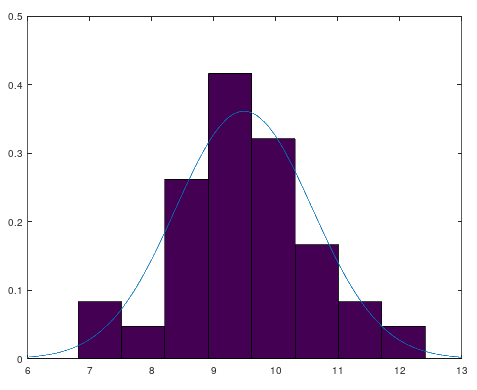
\includegraphics[scale=0.77]{pics/task1.png}}
	\caption{Гистограмма и график функции плотности распределения вероятностей нормальной случайной величины с математическим ожиданием $\hat\mu$ и дисперсией $S^2$}
\end{figure}

\begin{figure}[!h]
	\center{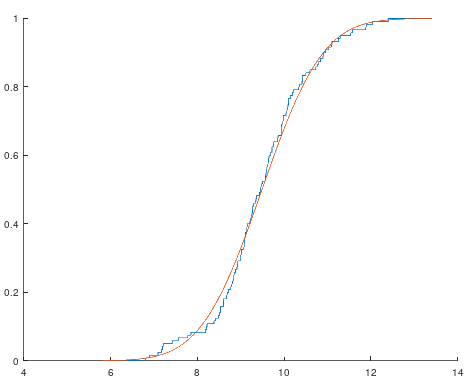
\includegraphics[scale=0.77]{pics/task2.png}}
	\caption{График эмпирической функции распределения и функции распределения нормальной случайной величины с математическим ожиданием $\hat\mu$ и дисперсией $S^2$}
\end{figure}

\end{document}